\documentclass[a4paper,11pt]{article}
\usepackage{amsmath, amsthm, amssymb, commath, graphicx, bbold, endnotes, graphicx, subfigure, multirow, setspace}
\usepackage[font=footnotesize]{caption}
\usepackage[top=1.25in, bottom=1.25in, left=1.25in, right=1.25in]{geometry}
\linespread{1}
\setlength{\parindent}{30pt}

\newcommand\fitparams{\boldsymbol{\theta}}
\newcommand\visfunc{\boldsymbol{\zeta}}
\newcommand\freqparams{\boldsymbol{\gamma}}
\newcommand\thermalcov{\boldsymbol{\mathsf{C}}_\text{T}}
\newcommand\modelcov{\boldsymbol{\mathsf{C}}_\text{M}}
\newcommand\modelcorr{\boldsymbol{\mathsf{C}}_\text{R}}
\newcommand\data{\boldsymbol{v}}
\newcommand\fisherinfo{\boldsymbol{\mathsf{I}}}
\newcommand\gains{\boldsymbol{g}}
\newcommand\gainsmat{\boldsymbol{\mathsf{G}}}
\newcommand\fitparamsu{\boldsymbol{u}}
\newcommand\modelvals{\boldsymbol{m}}
\newcommand\thermalvar{\boldsymbol{\sigma}_\text{T}^2}
\newcommand\modelvar{\boldsymbol{\sigma}_\text{M}^2}
\newcommand\matrixa{\boldsymbol{\mathsf{A}}}
\newcommand\uvcoord{\boldsymbol{x}}
\newcommand\beamvec{\boldsymbol{B}}
\newcommand\groundcoord{\boldsymbol{r}}
\newcommand\antres{\boldsymbol{b}}
\newcommand\beammat{\boldsymbol{\mathsf{B}}}
\newcommand\jonesmat{\boldsymbol{\mathsf{J}}}
\newcommand\coherency{\boldsymbol{\mathsf{S}}}
\newcommand\electricfield{\boldsymbol{E}}
\newcommand\vismat{\boldsymbol{\mathsf{V}}}
\newcommand\negloglikelihood{L}
\newcommand\truevis{\boldsymbol{w}}
\newcommand\modelnoise{\boldsymbol{n_\text{m}}}


\title{The Calibration Catalog}
\author{Ruby Byrne}
\date{March 2021}

\begin{document}

\maketitle

This memo discusses a compact source catalog that has been widely used for sky-based calibration of the Murchison Widefield Array (MWA) using the \textsc{fhd} software package, including in analysis of the Byrne et al.\ (in prep.) polarized diffuse map. Recently, the catalog has gained usage beyond \textsc{fhd}, motivating the creation of this memo to clarify the catalog contents.

\begin{figure}
\centering
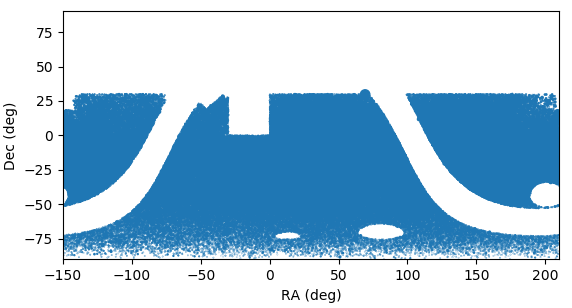
\includegraphics[width=4in]{GLEAM_all_plot.png}
\caption{}
\label{fig:gleam}
\end{figure}

The catalog is available in the \textsc{fhd} GitHub repository: \texttt{https://github.com/ EoRImaging/FHD/blob/master/catalog\_data/GLEAM\_v2\_plus\_rlb2019.sav}. It is based on the GLEAM point source catalog (Hurley-Walker et al.\ 2017). GLEAM is plotted as a scatter plot in Figure \ref{fig:gleam}. Notice that the catalog is missing fields near bright sources, doesn't include the galactic plane, and has a missing field from a corrupted night of data at the Northern edge of the catalog.

In addition to the obvious missing fields in the GLEAM catalog that we see in Figure \ref{fig:gleam}, the catalog is missing some of the brightest sources (including most of the so-called ``A-Team'' sources). In order to make this a workable catalog for calibration, we've supplemented it with models for those sources. The ``\texttt{GLEAM\_v2\_plus\_rlb2019.sav}'' catalog contains 9 additional sources not included in the GLEAM data release: 3C161, 3C409, Cassiopeia A, Centaurus A, Hera A, Hydra A, Pictor A, Virgo A, and Fornax A. These are listed in Table \ref{table}. 6 of these 9 sources are modeled as ``extended sources,'' meaning we do not approximate them as point sources but rather model some of their structure. In this catalog, that structure is modeled with pointlike components: an extended source is represented as a cluster of point sources.\footnote{There has been significant work in the field developing Gaussian or Shapelet source models, but \textsc{fhd} does not fully support those models yet. For that reason, we include pointlike source models only in this catalog. Nichole Barry and I have begun the process of getting \textsc{fhd} to read Gaussian source models correctly. For more information see this issue: \texttt{https://github.com/EoRImaging/FHD/issues/211}.} All of the 9 supplemented source models except for Fornax A were developed by Sarah White of the GLEAM collaboration. Fornax A was developed by Patricia Carroll.

\begin{table*}
\centering
\begin{tabular}{ |c|c|c|c|c| } 
 \hline
 \textbf{Name} & \textbf{Intensity} & \textbf{Comps.} & \textbf{Center RA} & \textbf{Center Dec.} \\ 
 \hline
 3C161 & 99.73 Jy & 1 & $96.8^\circ$ & $-5.9^\circ$ \\
 \hline 
 3C409 & 153.68 Jy & 1 & $303.6^\circ$ & $23.6^\circ$ \\
 \hline
 Cas. A & 17,693.90 Jy & 1 & $350.9^\circ$ & $58.8^\circ$ \\
 \hline
 Cen. A & 1,154.19 Jy & 5,874 & $201.6^\circ$ & $-43.5^\circ$ \\
 \hline
 Hera A & 279.36 Jy & 27 & $252.7^\circ$ & $5.0^\circ$ \\
 \hline
 Hyd. A & 226.32 Jy & 58 & $139.5^\circ$ & $-12.1^\circ$ \\
 \hline
 Pic. A & 271.16 Jy & 88 & $80.0^\circ$ & $-45.8^\circ$ \\
 \hline
 Vir. A & 372.73 Jy & 171 & $187.7^\circ$ & $12.4^\circ$ \\
 \hline
 For. A & 541.77 Jy & 1,924 & $50.6^\circ$ & $-37.2^\circ$ \\
 \hline
\end{tabular}
\caption{}
\label{table}
\end{table*}

This catalog contains 307,464 sources. It is designed to work in the MWA's EoR ``high band,'' centered at 182 MHz, and does not include any spectral index information.

The catalog is stored as an \textsc{fhd}-readable IDL save file. It can be easily read with the \textsc{pyradiosky} Python package,\footnote{\texttt{https://github.com/RadioAstronomySoftwareGroup/pyradiosky}} which offers a well-documented Python interface for astrophysical source catalogs. To read this catalog with \textsc{pyradiosky}, use the \texttt{read\_fhd\_catalog} function.


\end{document}